\documentclass{beamer}
\usepackage{textpos}
%\input{Theme/Packages.tex}
\usetheme{Madrid}
\usecolortheme{beaver}
\usepackage{siunitx} % Zahlen, Einheiten und Tabellenformatierung
	\sisetup{
		locale = DE,
		per-mode = symbol,
		output-decimal-marker = {.},
		separate-uncertainty = true,
		binary-units = true
	}
\usepackage[backend=biber,sorting=none, style=authoryear]{biblatex}
\addbibresource{Bib/Full_Bibliography.bib}
\beamertemplatenavigationsymbolsempty
\title{Selection on loss-of-function variants}
\titlegraphic{
\includegraphics[scale=0.3]{images/CCTB_Logo.pdf}}
\author{Laura Steinmann}
\date{06.04.2022}

\begin{document}
\addtobeamertemplate{frametitle}{}{%
\begin{textblock*}{10mm}(0.851\textwidth,-1.0cm)

\includegraphics[height=1cm,width=1.2cm]{images/Uni-Wuerzburg.jpg}
\end{textblock*}
\begin{textblock*}{100mm}(0.95\textwidth,-1cm)

\includegraphics[height=1cm,width=1.0cm]{images/CCTB_short_logo.jpeg}
\end{textblock*}

}

{\setbeamertemplate{footline}{}
\frame{\titlepage}}
\begin{frame}{Natural variation in \textit{Arabidopsis thaliana} \footcite{Durufle2019}}
\begin{figure}[tb]
	\centering
	\begin{minipage}[h]{1\textwidth}
	\centering
	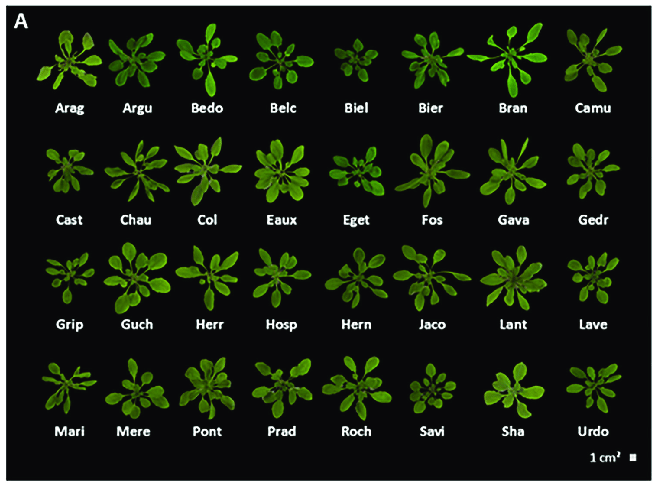
\includegraphics[width=0.75\textwidth]{images/Natural_Variation.png}
	\label{fig:Natural_Variation}
	\end{minipage}
\end{figure}
\end{frame}
\section{Introduction}
\begin{frame}[plain]
    \vfill
    \centering
    \begin{beamercolorbox}[sep=8pt,center,shadow=true,rounded=true]{title}
      \usebeamerfont{title}\insertsectionhead\par%
      \noindent\rule{10cm}{1pt} \\
    \end{beamercolorbox}
    \vfill
\end{frame}
\begin{frame}{Fundamental process of adaptation:\\ DNA mutations \footcite{bresch2013}}
	\textbf{Point Mutations}
	\begin{figure}[tb]
		\centering
		\begin{minipage}[h]{1\textwidth}
		\centering
		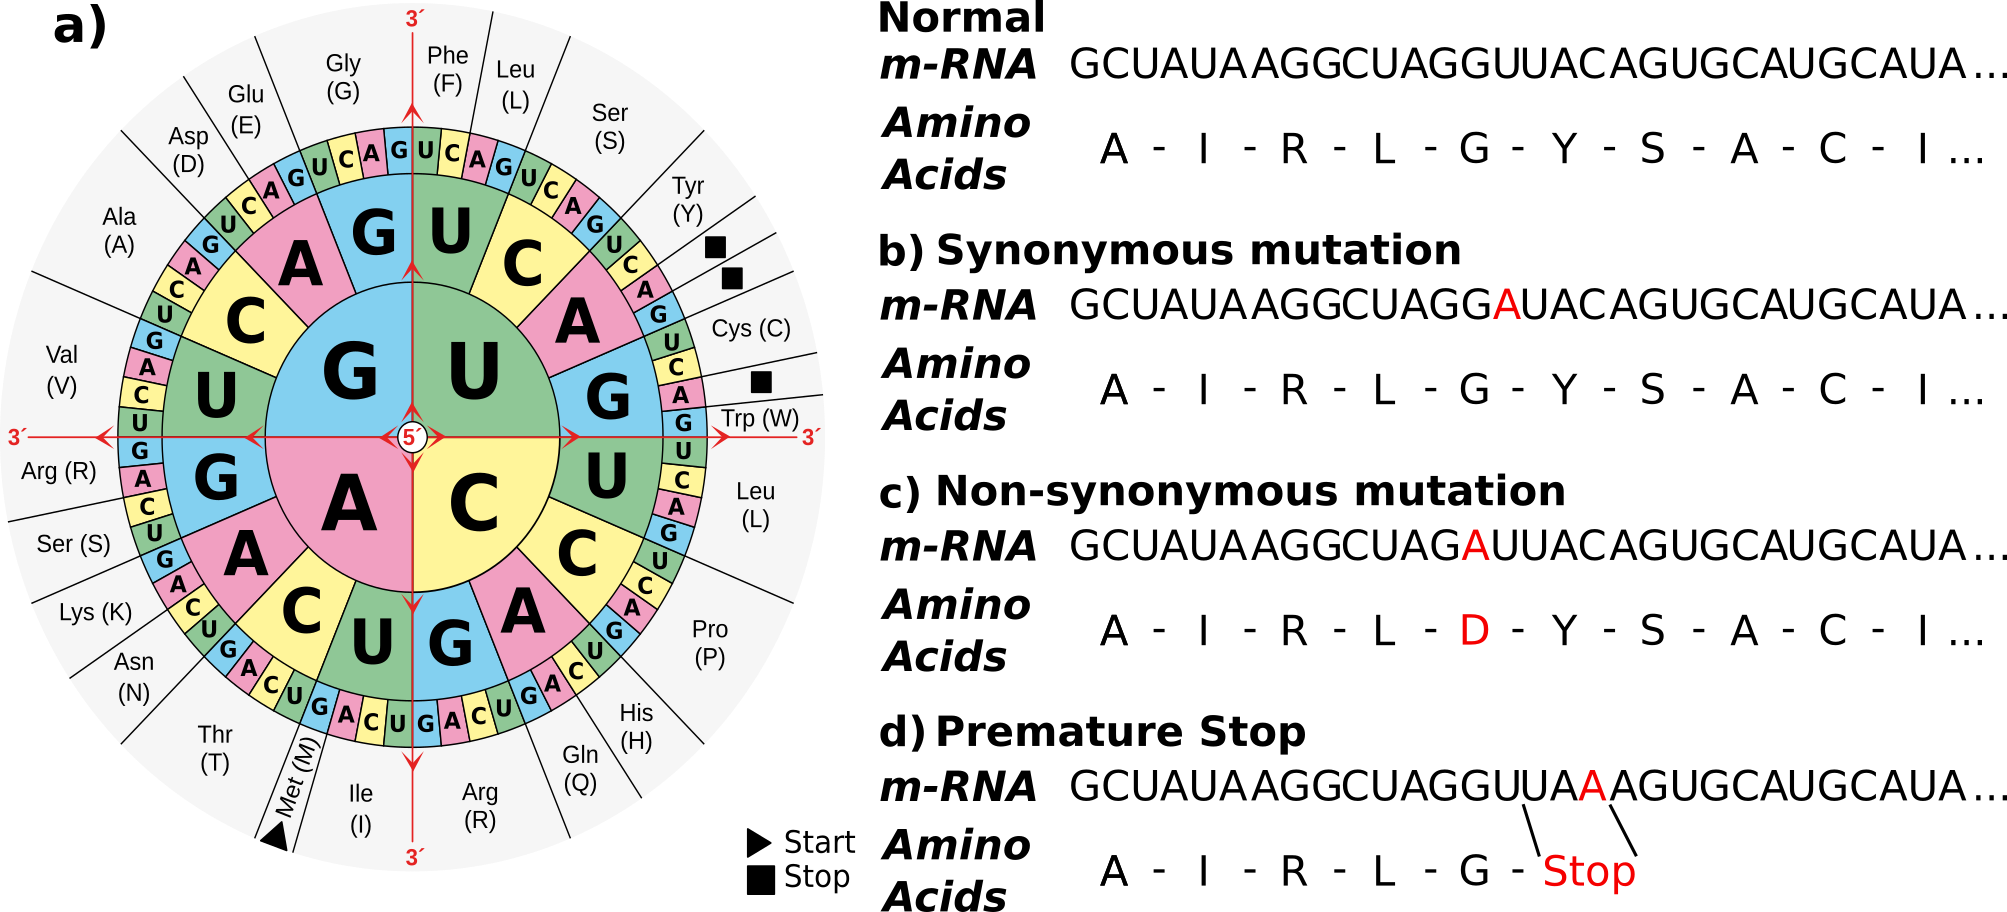
\includegraphics[width=0.9\textwidth]{images/Mutations.png}
		\label{fig:Mutations}
		\end{minipage}
	\end{figure}
\end{frame}
\begin{frame}{Point Mutations on population scale}
	\begin{itemize}
		\item Point mutations, which occur on population scale and differ between individuals are called \textbf{single nucleotide polymorphisms}
		\item After emergence of a mutation natural selection acts on them and influence their presence in the populations genetic pool 
		\begin{itemize}
			\item[$\rightarrow$] Fatal mutations were removed from the genetic pool
			\item[$\rightarrow$] Mutations with positive impact are preserved and accumulated in the genetic pool
			\item[$\rightarrow$] Neutral mutations are not shaped by natural selection
		\end{itemize}
	\end{itemize}
\end{frame}	
\begin{frame}{Premature stop codons on gene regulatory \\networks \footcite{Yao2021}}
	\begin{figure}[tb]
		\centering
		\begin{minipage}[h]{1\textwidth}
		\centering
		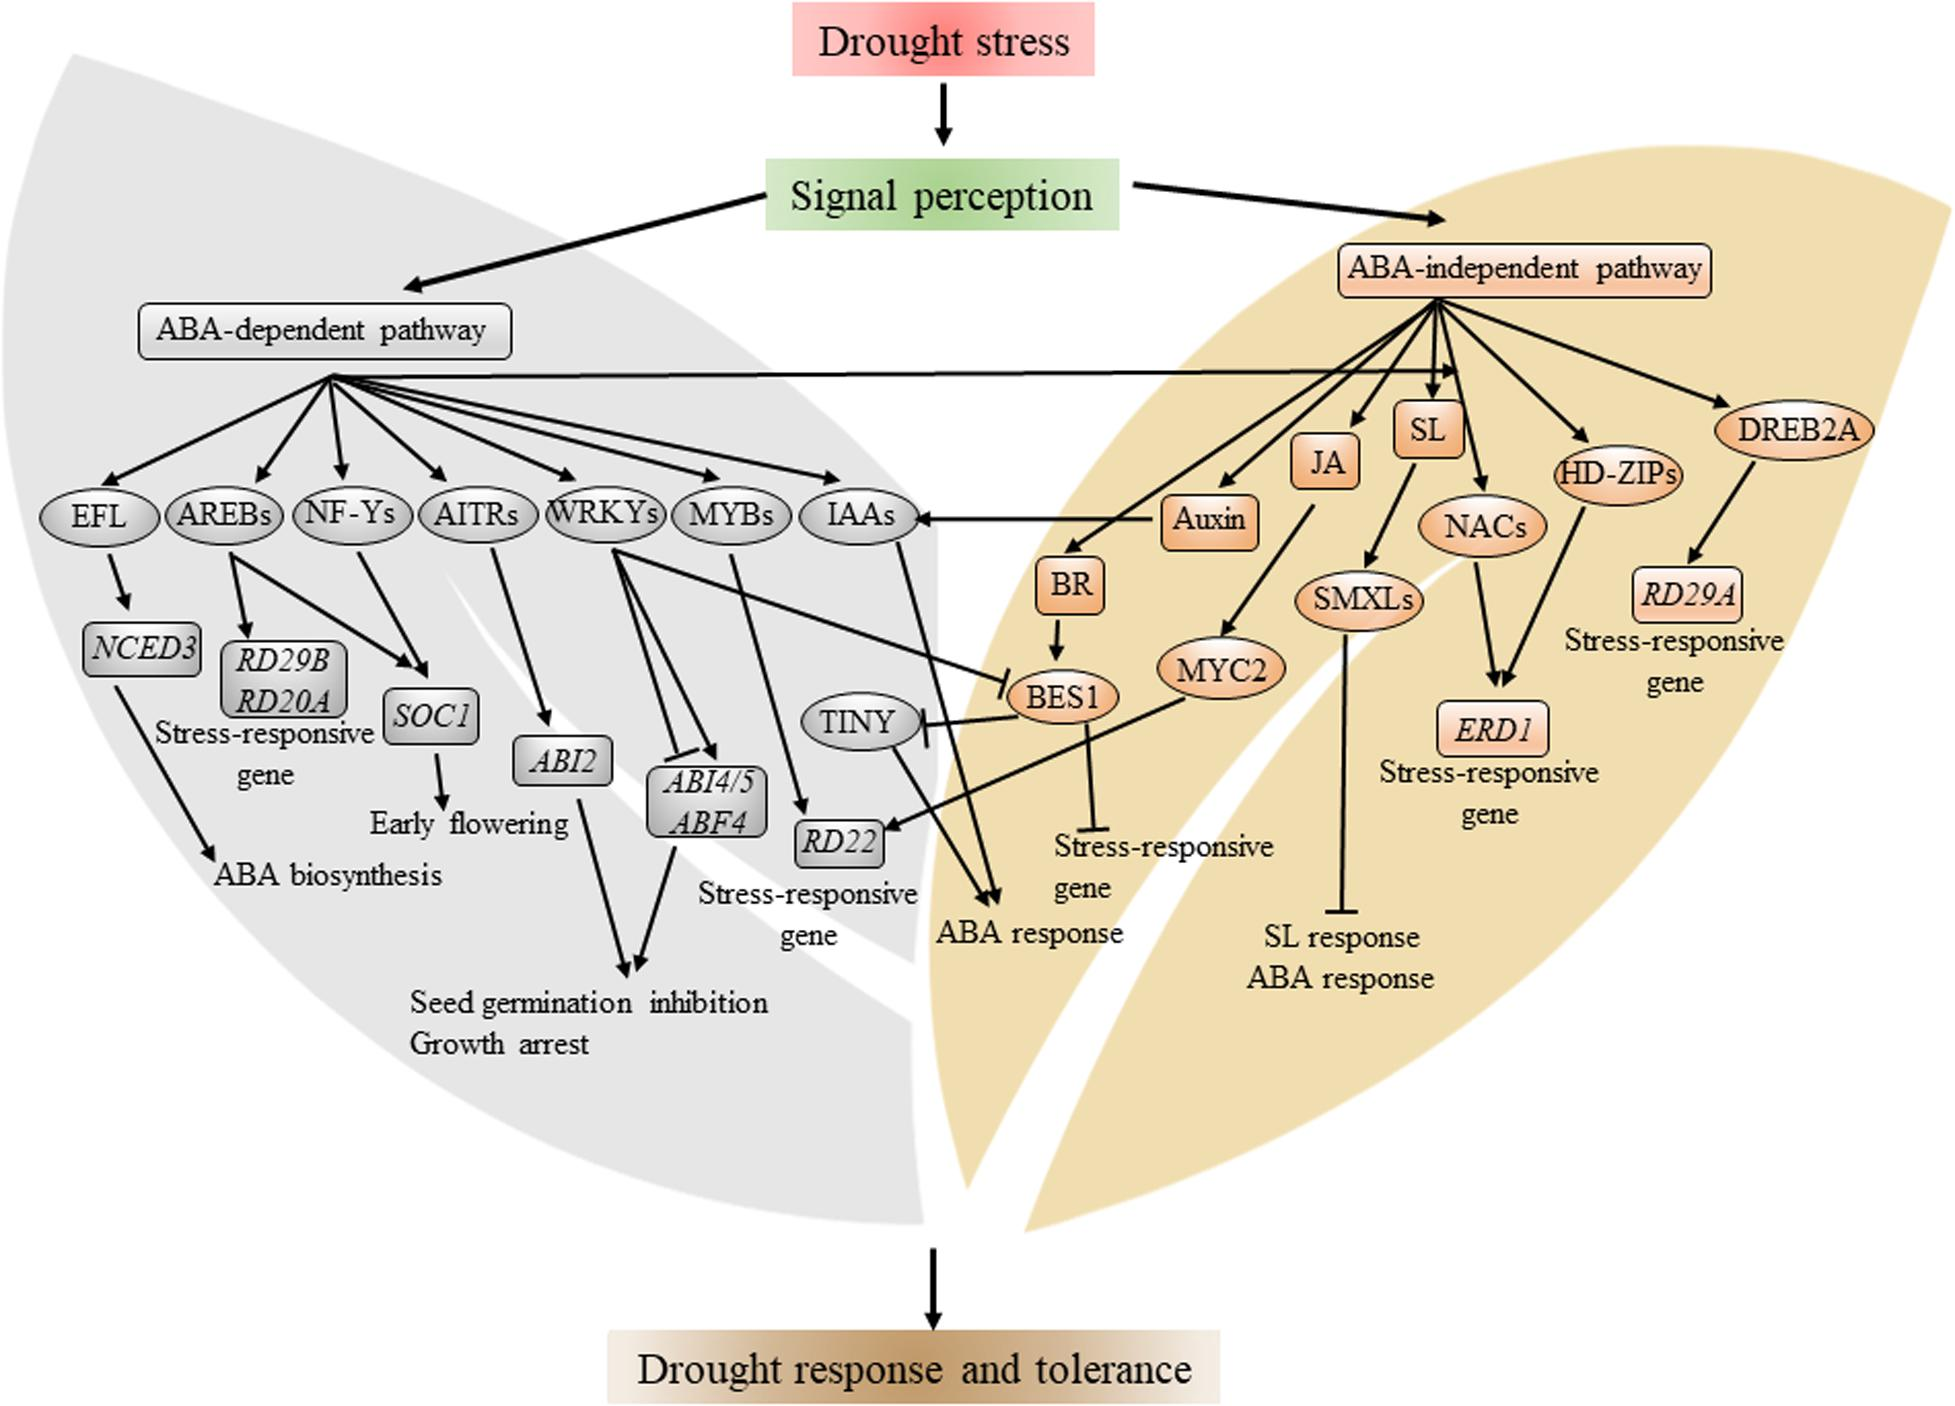
\includegraphics[width=0.8\textwidth]{images/ABA_Network.jpg}
		\label{fig:Example_Network}
		\end{minipage}
	\end{figure}
\end{frame}
\begin{frame}{Premature stop codons on gene regulatory \\networks \footcite{Yao2021}}
	\begin{figure}[tb]
		\centering
		\begin{minipage}[h]{1\textwidth}
		\centering
		\includegraphics[width=0.8\textwidth]{images/Knock_out_network.png}
		\label{fig:Example_Network_with_knock_out}
		\end{minipage}
	\end{figure}
\end{frame}
\begin{frame}{Premature stop codons on gene regulatory \\networks \footcite{Yao2021}}
	\begin{figure}[tb]
		\centering
		\begin{minipage}[h]{1\textwidth}
		\centering
		\includegraphics[width=0.8\textwidth]{images/Knock_out_network_II.png}
		\label{fig:Example_Network_with_knock_outII}
		\end{minipage}
	\end{figure}
\end{frame}
\section{Dataset of Arabidopsis thaliana}
\begin{frame}[plain]
    \vfill
    \centering
    \begin{beamercolorbox}[sep=8pt,center,shadow=true,rounded=true]{title}
      \usebeamerfont{title}\insertsectionhead\par%
      \noindent\rule{10cm}{1pt} \\
    \end{beamercolorbox}
    \vfill
\end{frame}
\begin{frame}{1001 Genomes Project of \textit{A. thaliana}}
	\begin{itemize}
		\item 1,135 ecotypes (accessions) of \textit{A. thaliana} with full sequenced genomes 
	\end{itemize}
\end{frame}
\begin{frame}{1001 Genomes Project of \textit{A. thaliana}\footcite{1001Genomes2016}}
	\begin{figure}[tb]
		\centering
		\begin{minipage}[h]{1\textwidth}
		\centering
		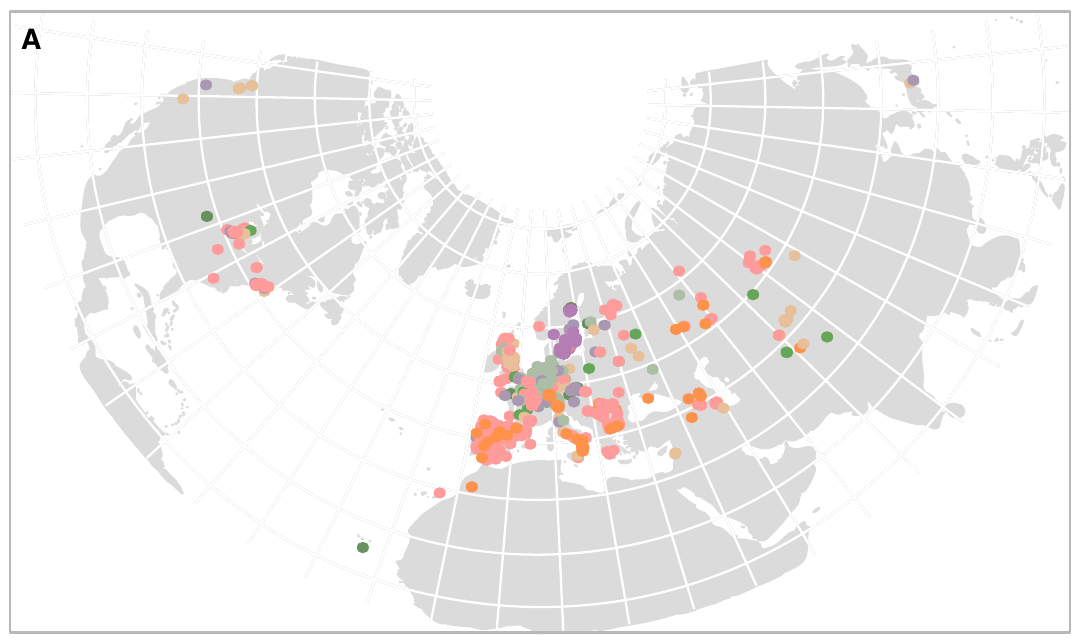
\includegraphics[width=0.8\textwidth]{images/Origins_1001_Genomes.png}
		\label{fig:Origins_1135}
		\end{minipage}
	\end{figure}
\end{frame}
\begin{frame}{1001 Genomes Project of \textit{A. thaliana}}
	\begin{itemize}
		\item 1,135 ecotypes (accessions) of \textit{A. thaliana} with full sequenced genomes 
		\begin{itemize}
			\item 10,707,430 SNPs detected in this population
		\end{itemize}
		\item Transcriptomes of 727 accessions were sequenced 
		\item[$\rightarrow$] For \textbf{665 accessions} genomic and transcriptomic information is available 
	\end{itemize}
\end{frame}
\section{Project idea}
\begin{frame}[plain]
    \vfill
    \centering
    \begin{beamercolorbox}[sep=8pt,center,shadow=true,rounded=true]{title}
      \usebeamerfont{title}\insertsectionhead\par%
      \noindent\rule{10cm}{1pt} \\
    \end{beamercolorbox}
    \vfill
\end{frame}
\begin{frame}{Project: Selection on loss-of-function variants}
	\textbf{How is natural selection shaping population structures through loss-of-function variants?}

	\vspace{3mm}
	\begin{itemize}
		\item Studying attributes and occurrence of premature stop codons in the 1,135 population of \textit{A. thaliana} 
		\item Generating two high confidential datasets for further analysis
		\begin{itemize}
			\item[-] Approach 1: Gene expression differences between wildtype and knock-out accessions 
			\item[-] Approach 2: Remaining length of the protein 
		\end{itemize}
		\item Studying interactions between premature stop codons
		\item Comparing these findings to a control group
	\end{itemize}
\end{frame}
\section{Results}
\begin{frame}[plain]
    \vfill
    \centering
    \begin{beamercolorbox}[sep=8pt,center,shadow=true,rounded=true]{title}
      \usebeamerfont{title}\insertsectionhead\par%
      \noindent\rule{10cm}{1pt} \\
    \end{beamercolorbox}
    \vfill
\end{frame}
\begin{frame}{Distribution of premature stop codons across \\ accessions}
	\begin{figure}[tb]
		\centering
		\begin{minipage}[h]{1\textwidth}
		\centering
		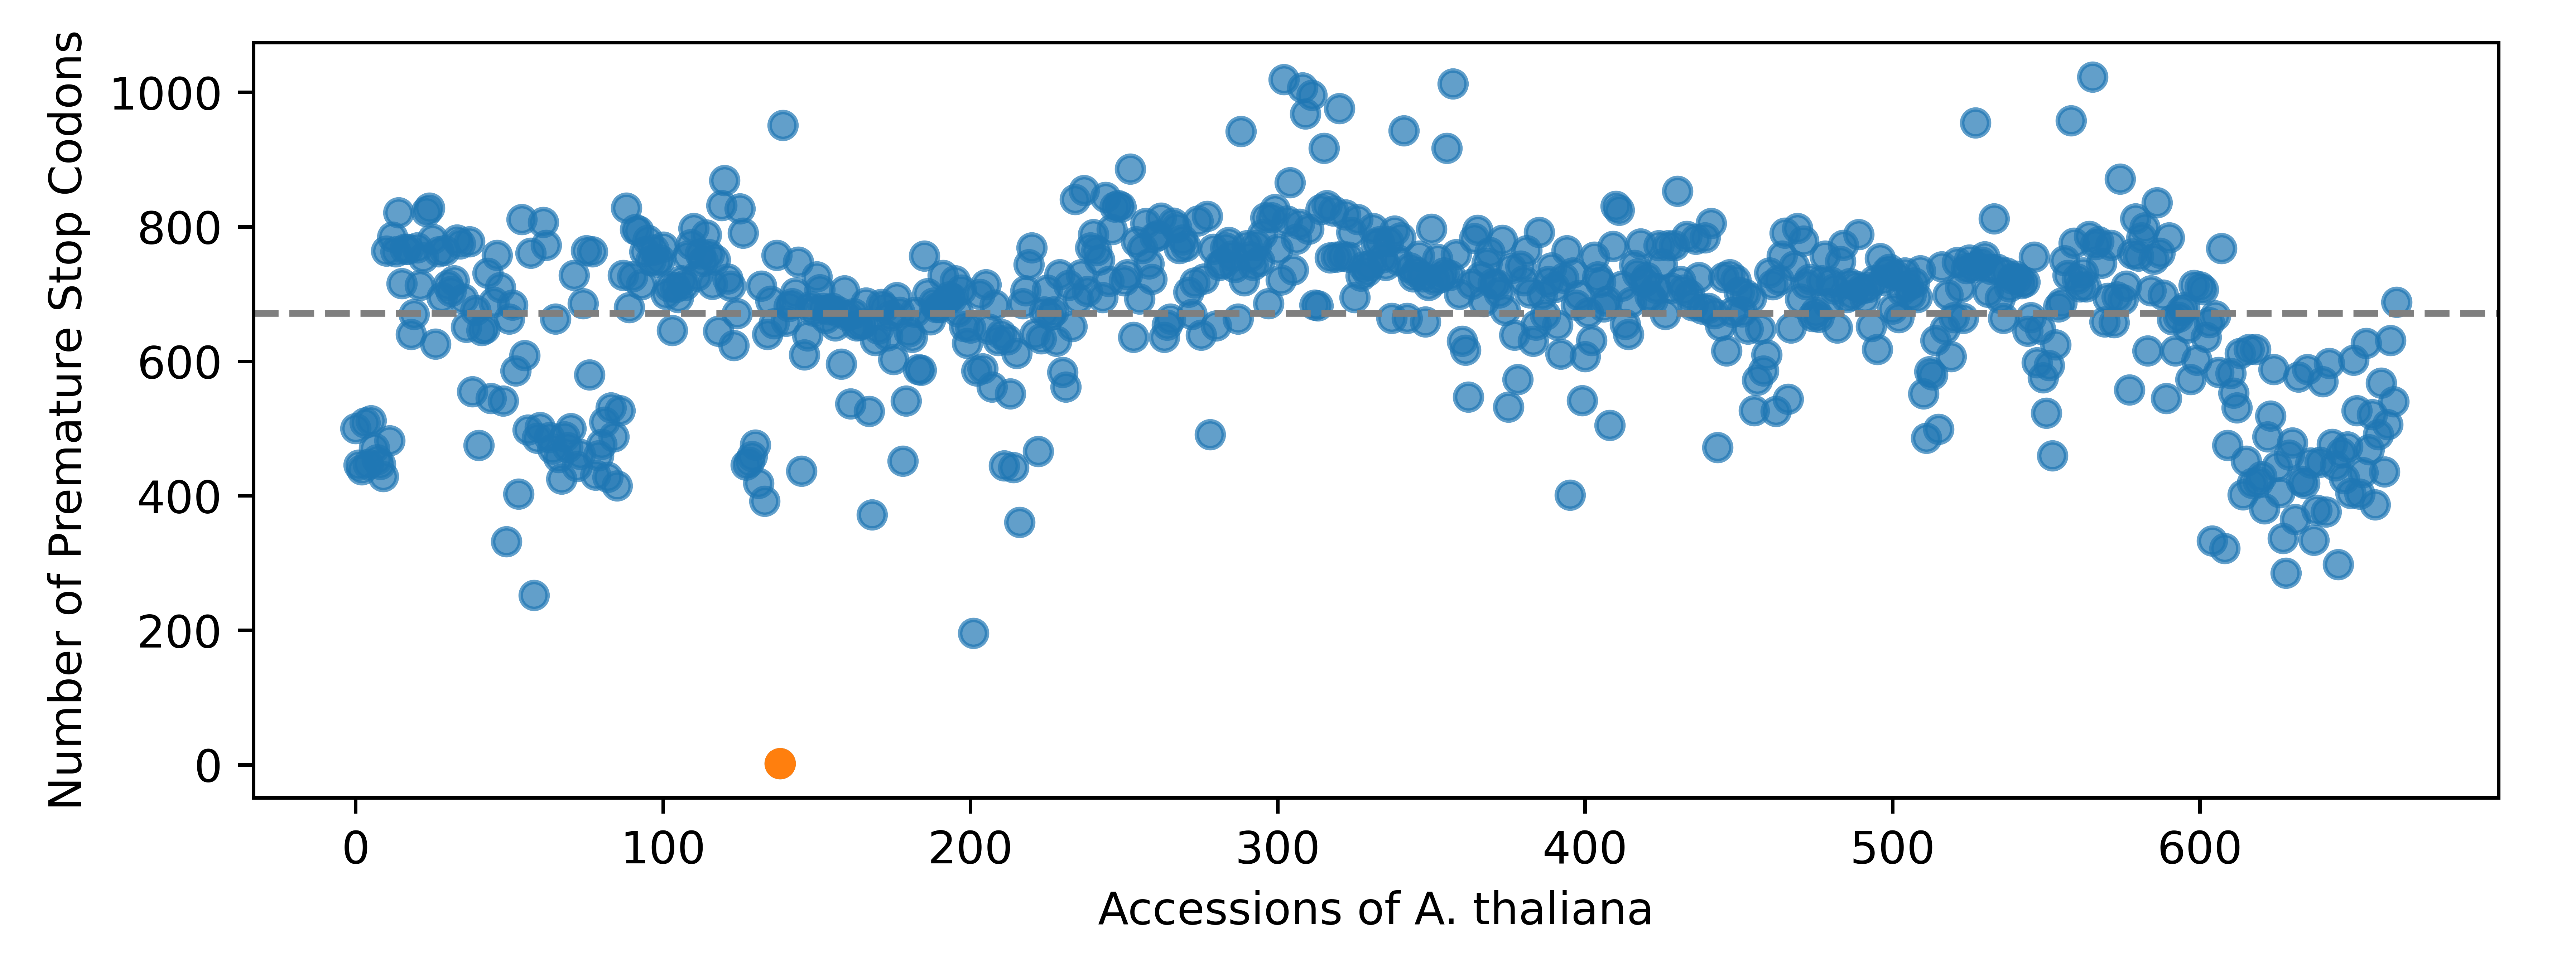
\includegraphics[width=1\textwidth]{images/Distribution_Premature_Stop_CodonsI.png}
		\label{fig:Distribution_Premature_Stop_CodonsI}
		\end{minipage}
	\end{figure}
	\begin{itemize}
		\item On average 671 premature stop codons detected in an accession
		\item Exception col-0 (orange) $\rightarrow$ the reference genome 
		\item Maximum of 1023 premature stop codon in one single accession
	\end{itemize}
\end{frame}
\begin{frame}{Distribution of premature stop codons across \\ genes}
	\begin{figure}[tb]
		\centering
		\begin{minipage}[h]{1\textwidth}
		\centering
		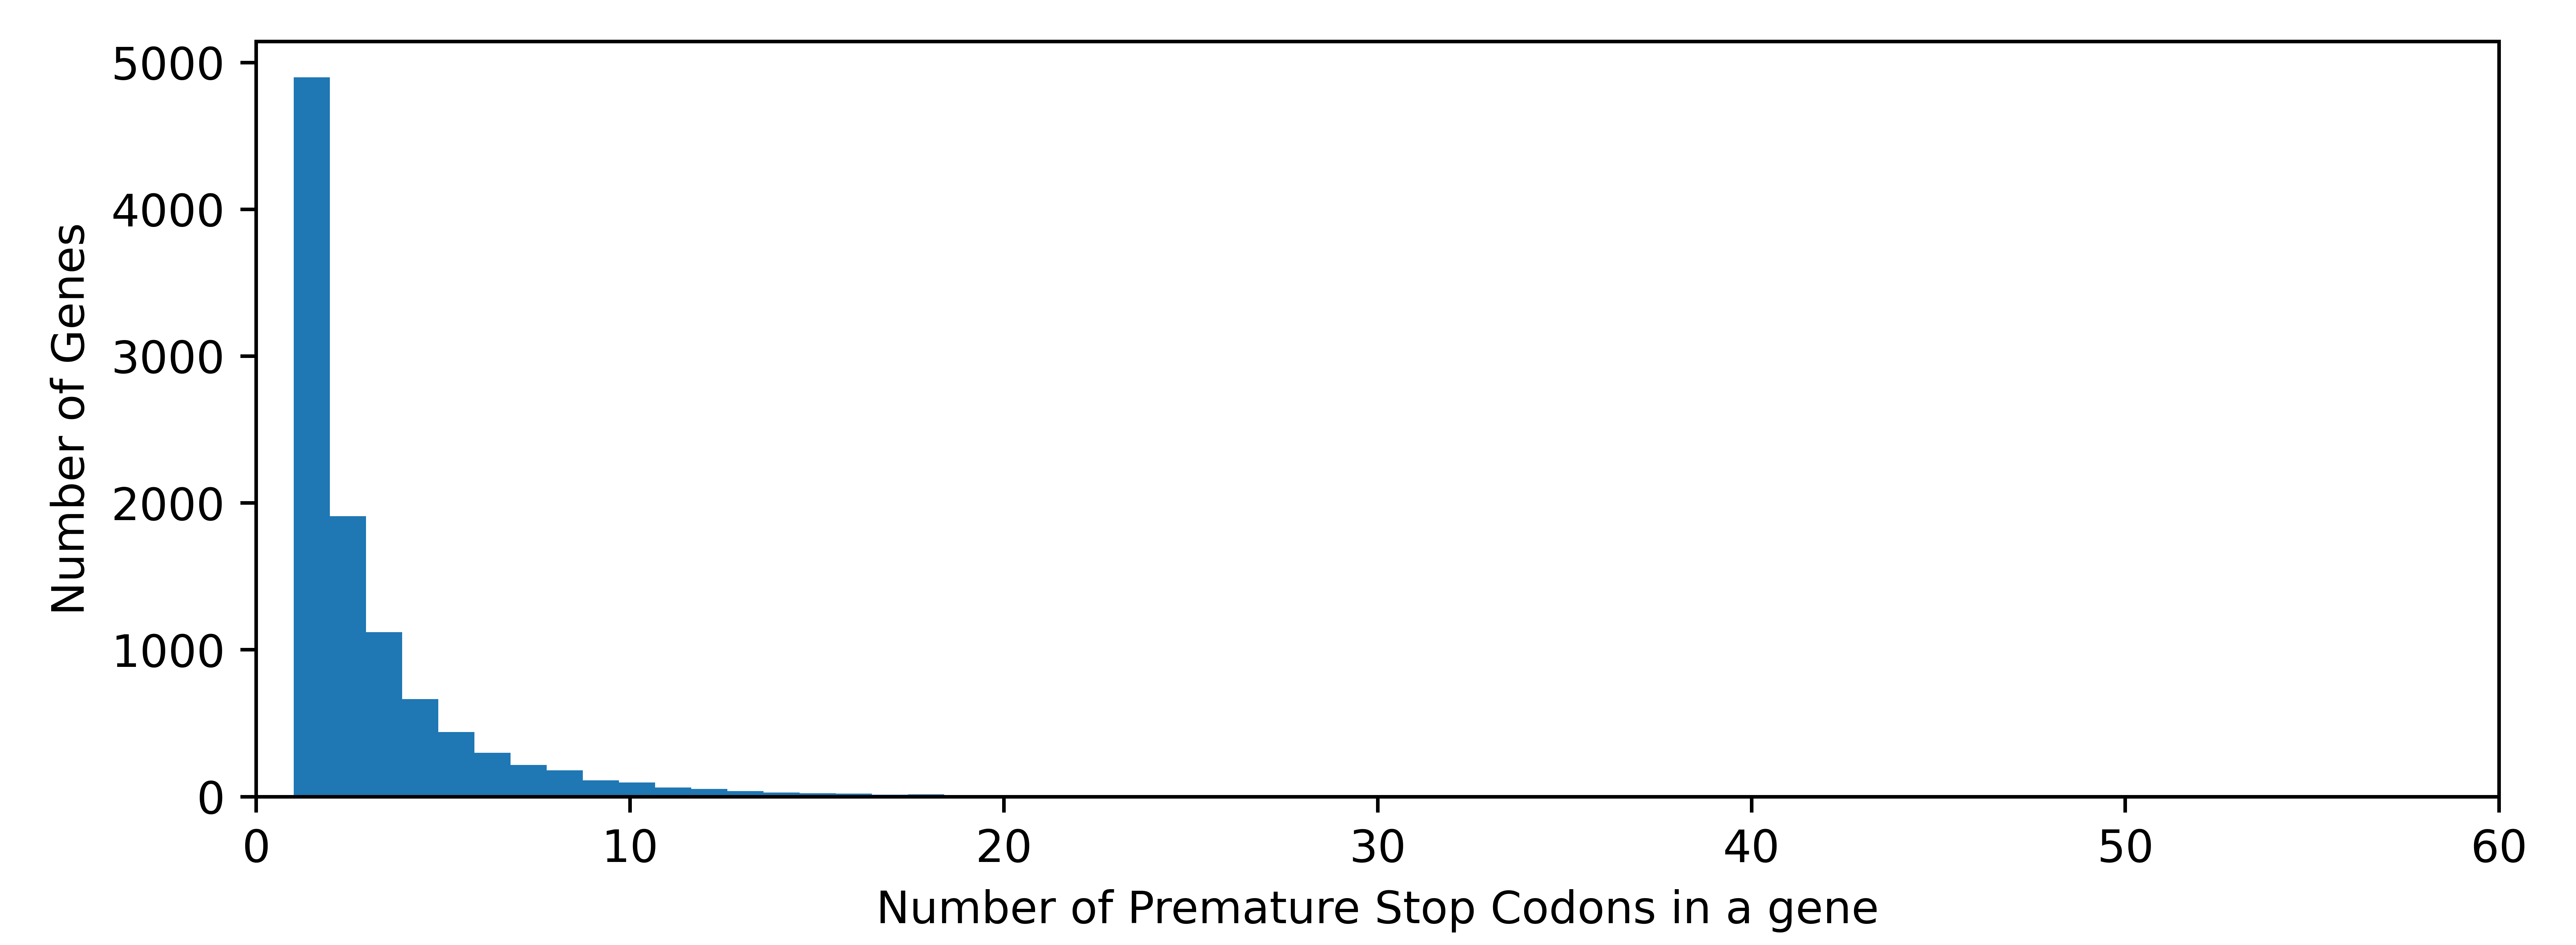
\includegraphics[width=1\textwidth]{images/Distribution_Premature_Stop_CodonsII.png}
		\label{fig:Distribution_Premature_Stop_CodonsII}
		\end{minipage}
	\end{figure}
	\begin{itemize}
		\item Roughly half of the genes is knocked out with a single premature stop codon 
		\item Unexpected findings of up to 59 stop codons in a single gene
		\begin{itemize}
			\item[$\rightarrow$] Population structure
			\item[$\rightarrow$] Splicing variants 
		\end{itemize}
	\end{itemize}
\end{frame}
\section{Generation of high confidential dataset}
\begin{frame}[plain]
    \vfill
    \centering
    \begin{beamercolorbox}[sep=8pt,center,shadow=true,rounded=true]{title}
      \usebeamerfont{title}\insertsectionhead\par%
      \noindent\rule{10cm}{1pt} \\
    \end{beamercolorbox}
    \vfill
\end{frame}
\begin{frame}{Approach 1: Gene expression differences}
	\textbf{Method}

	analysis of just 665 accessions, for which we have genomic and transcriptomic information
	
	\vspace{5mm}
	\begin{enumerate}
		\item[1.)] Filter according to information of the overlapping datasets
	\end{enumerate}
\end{frame}
\begin{frame}{Approach 1: Gene expression differences}
	\textbf{Method}

	analysis of just 665 accessions, for which we have genomic and transcriptomic information
	
	\vspace{5mm}
	\begin{enumerate}
		\item[1.)] Filter according to information of the overlapping datasets
		\item[2.)] Classify each accessions as wildtype (without premature stop codon) or knock-out accession (with premature stop codon) for each premature stop codon
	\end{enumerate}
\end{frame}
\begin{frame}{Approach 1: Gene expression differences}
	\textbf{Method}

	analysis of just 665 accessions, for which we have genomic and transcriptomic information
	
	\vspace{5mm}
	\begin{enumerate}
		\item[1.)] Filter according to information of the overlapping datasets
		\item[2.)] Classify each accessions as wildtype (without premature stop codon) or knock-out accession (with premature stop codon) for each premature stop codon
		\item[3.)] Calculate a t-test to classify premature stop codons into three different groups
		\begin{itemize}
			\item Unsignificant change of gene expression
			\item Significant decrease of gene expression 
			\item Significant increase of gene expression
		\end{itemize}  
	\end{enumerate}
\end{frame}
\begin{frame}{Approach 1: Gene expression differences}
	\begin{figure}[tb]
		\centering
		\begin{minipage}[h]{1\textwidth}
		\centering
		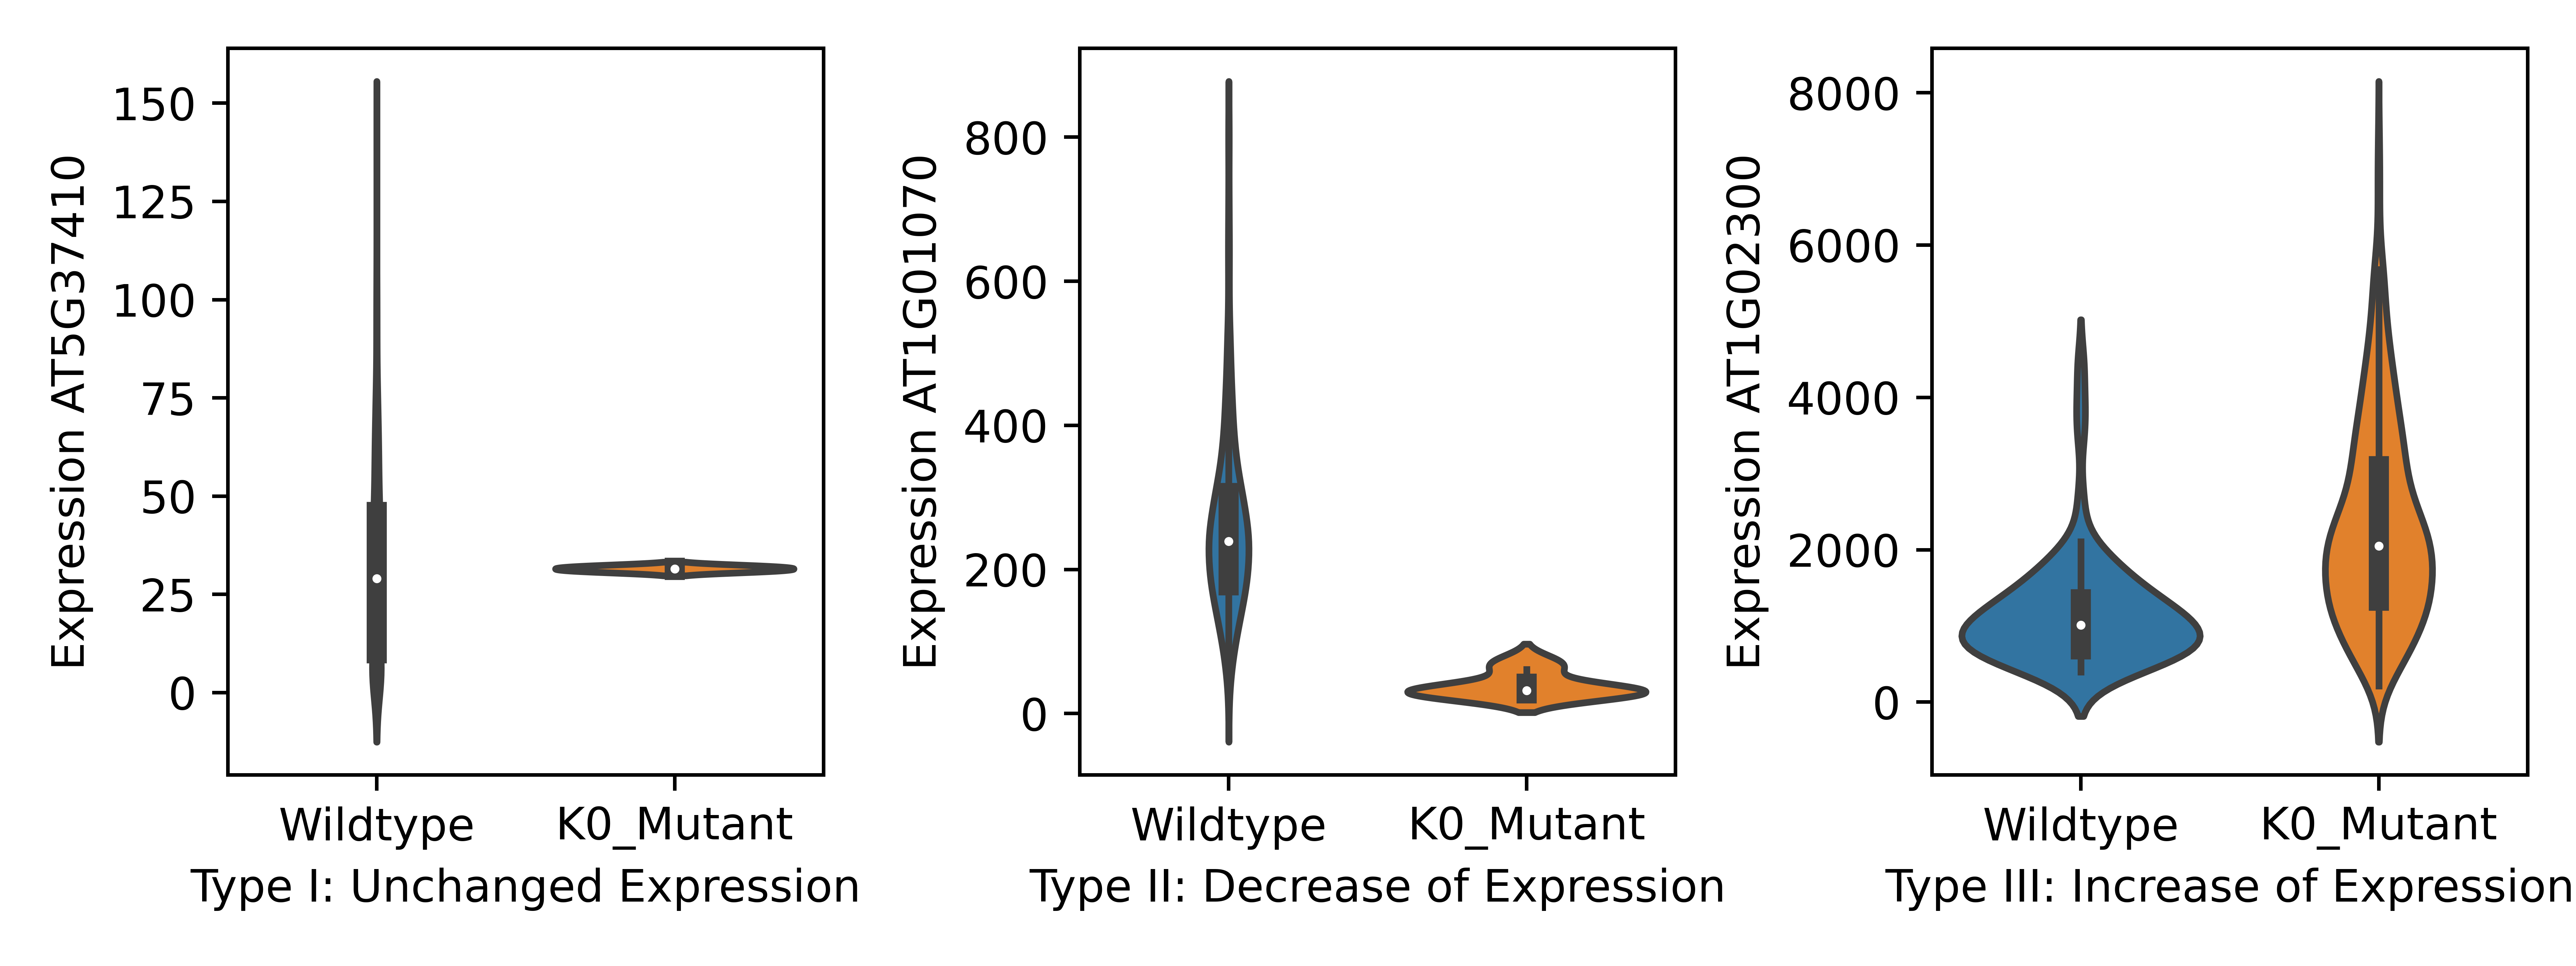
\includegraphics[width=1\textwidth]{images/Cathegories_Premature_Stop_Codons.png}
		\label{fig:Cathegories}
		\end{minipage}
	\end{figure}
\end{frame}
\begin{frame}{Approach 1: Gene expression differences}
	\begin{figure}[tb]
		\centering
		\begin{minipage}[h]{1\textwidth}
		\centering
		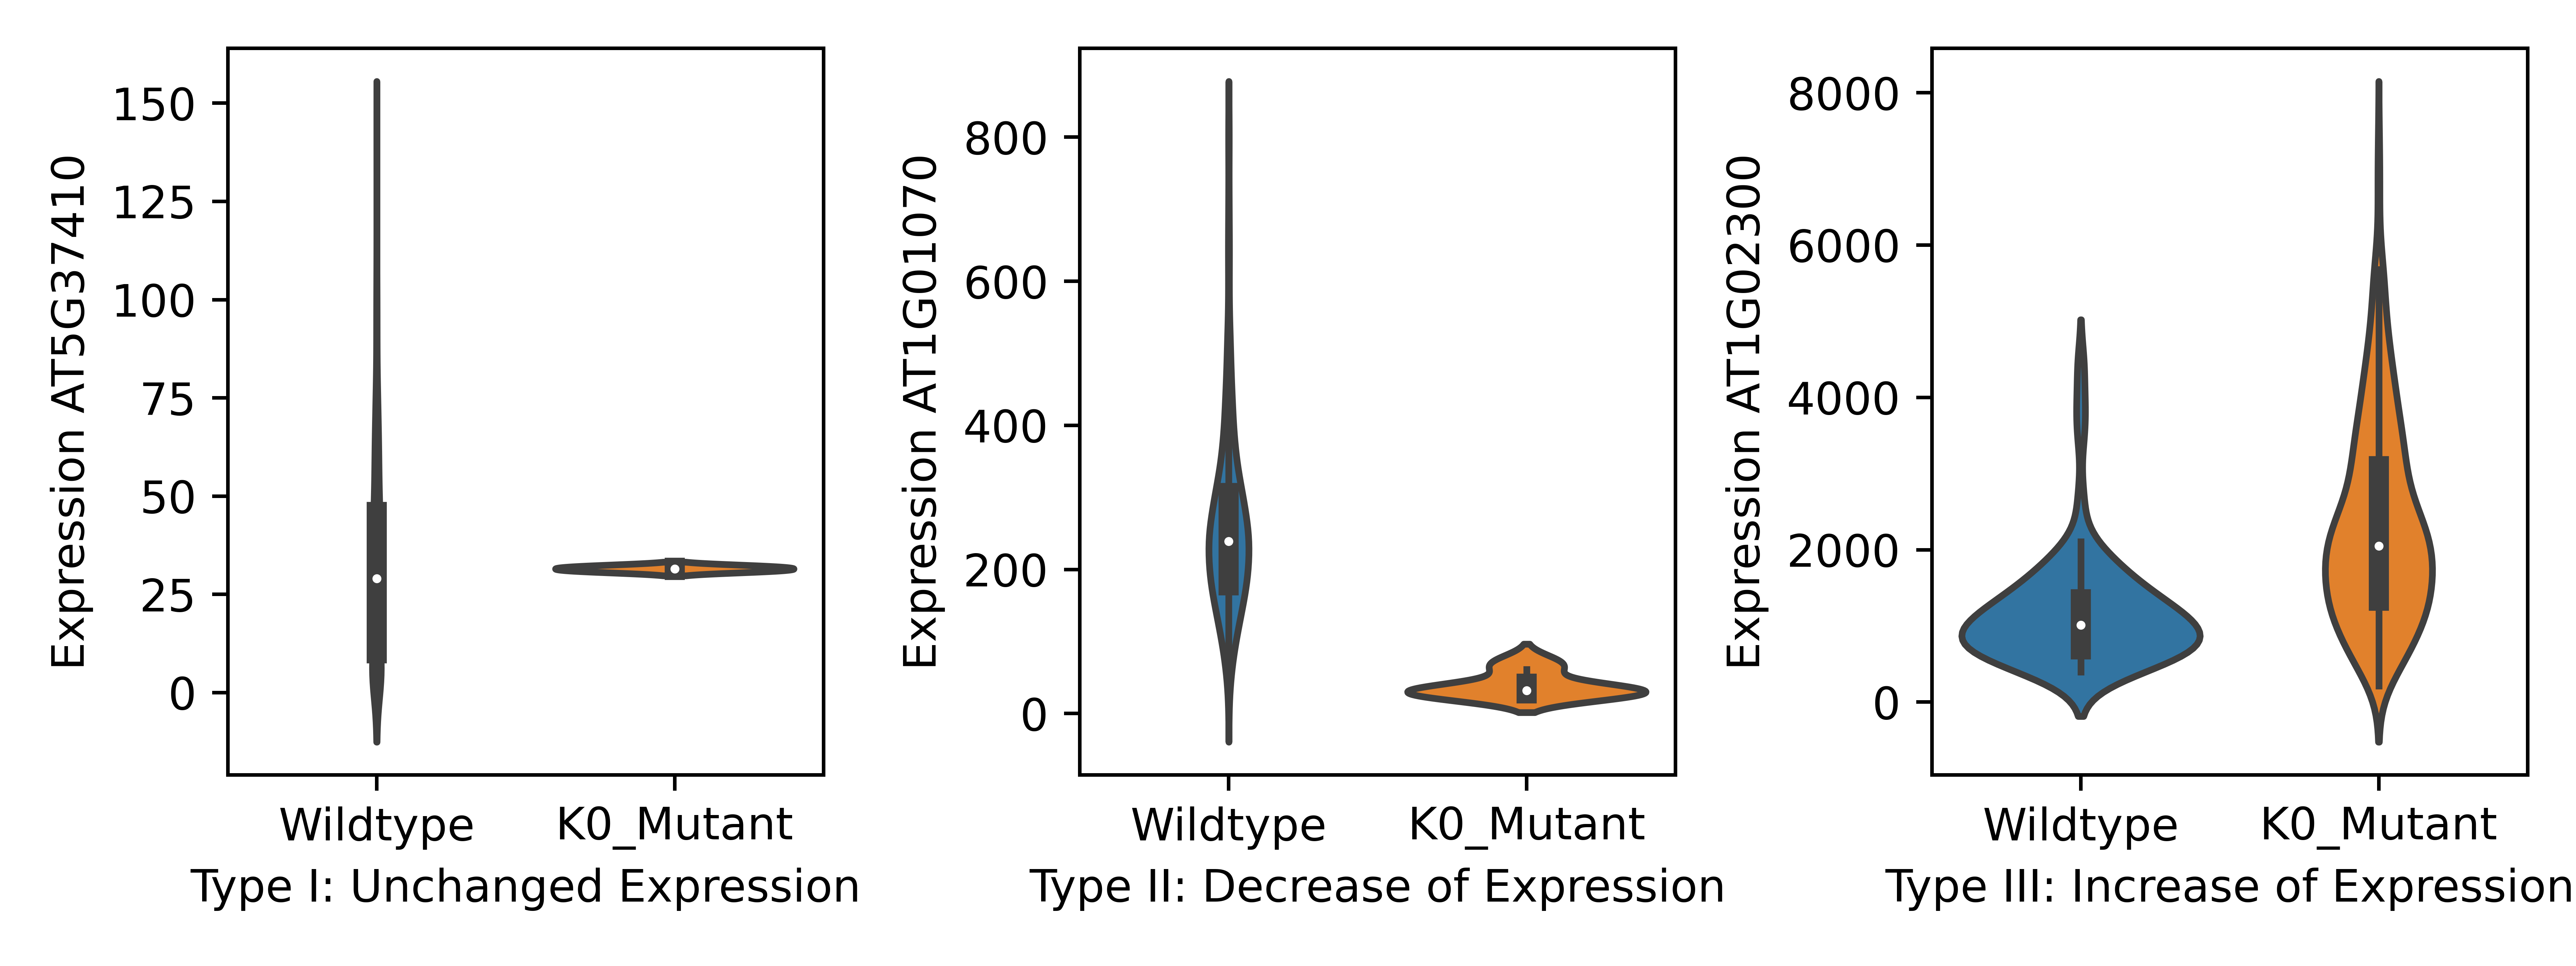
\includegraphics[width=1\textwidth]{images/Cathegories_Premature_Stop_Codons.png}
		\label{fig:Cathegories}
		\end{minipage}
	\end{figure}
	\begin{table}[tb]
		\label{tab:Categories}
		\centering
		\begin{tabular}{|l|l|l|l|}
		\hline
		\begin{tabular}[c]{@{}l@{}} \textbf{p-value} \\ \textbf{threshold} \end{tabular} & \begin{tabular}[c]{@{}l@{}} \textbf{Type I} \end{tabular} & \begin{tabular}[c]{@{}l@{}} \textbf{Type II} \end{tabular} & \begin{tabular}[c]{@{}l@{}}\textbf{Type III} \end{tabular} \\ \hline
		0.05 & 5433 & 949 & 742 \\ \hline
		bonferroni & 6608 & 247 & 269 \\ \hline
		\end{tabular}
		\end{table}                  
\end{frame}
\begin{frame}{Approach 2: Remaining length of the protein}
	\begin{figure}[tb]
		\centering
		\begin{minipage}[h]{1\textwidth}
		\centering
		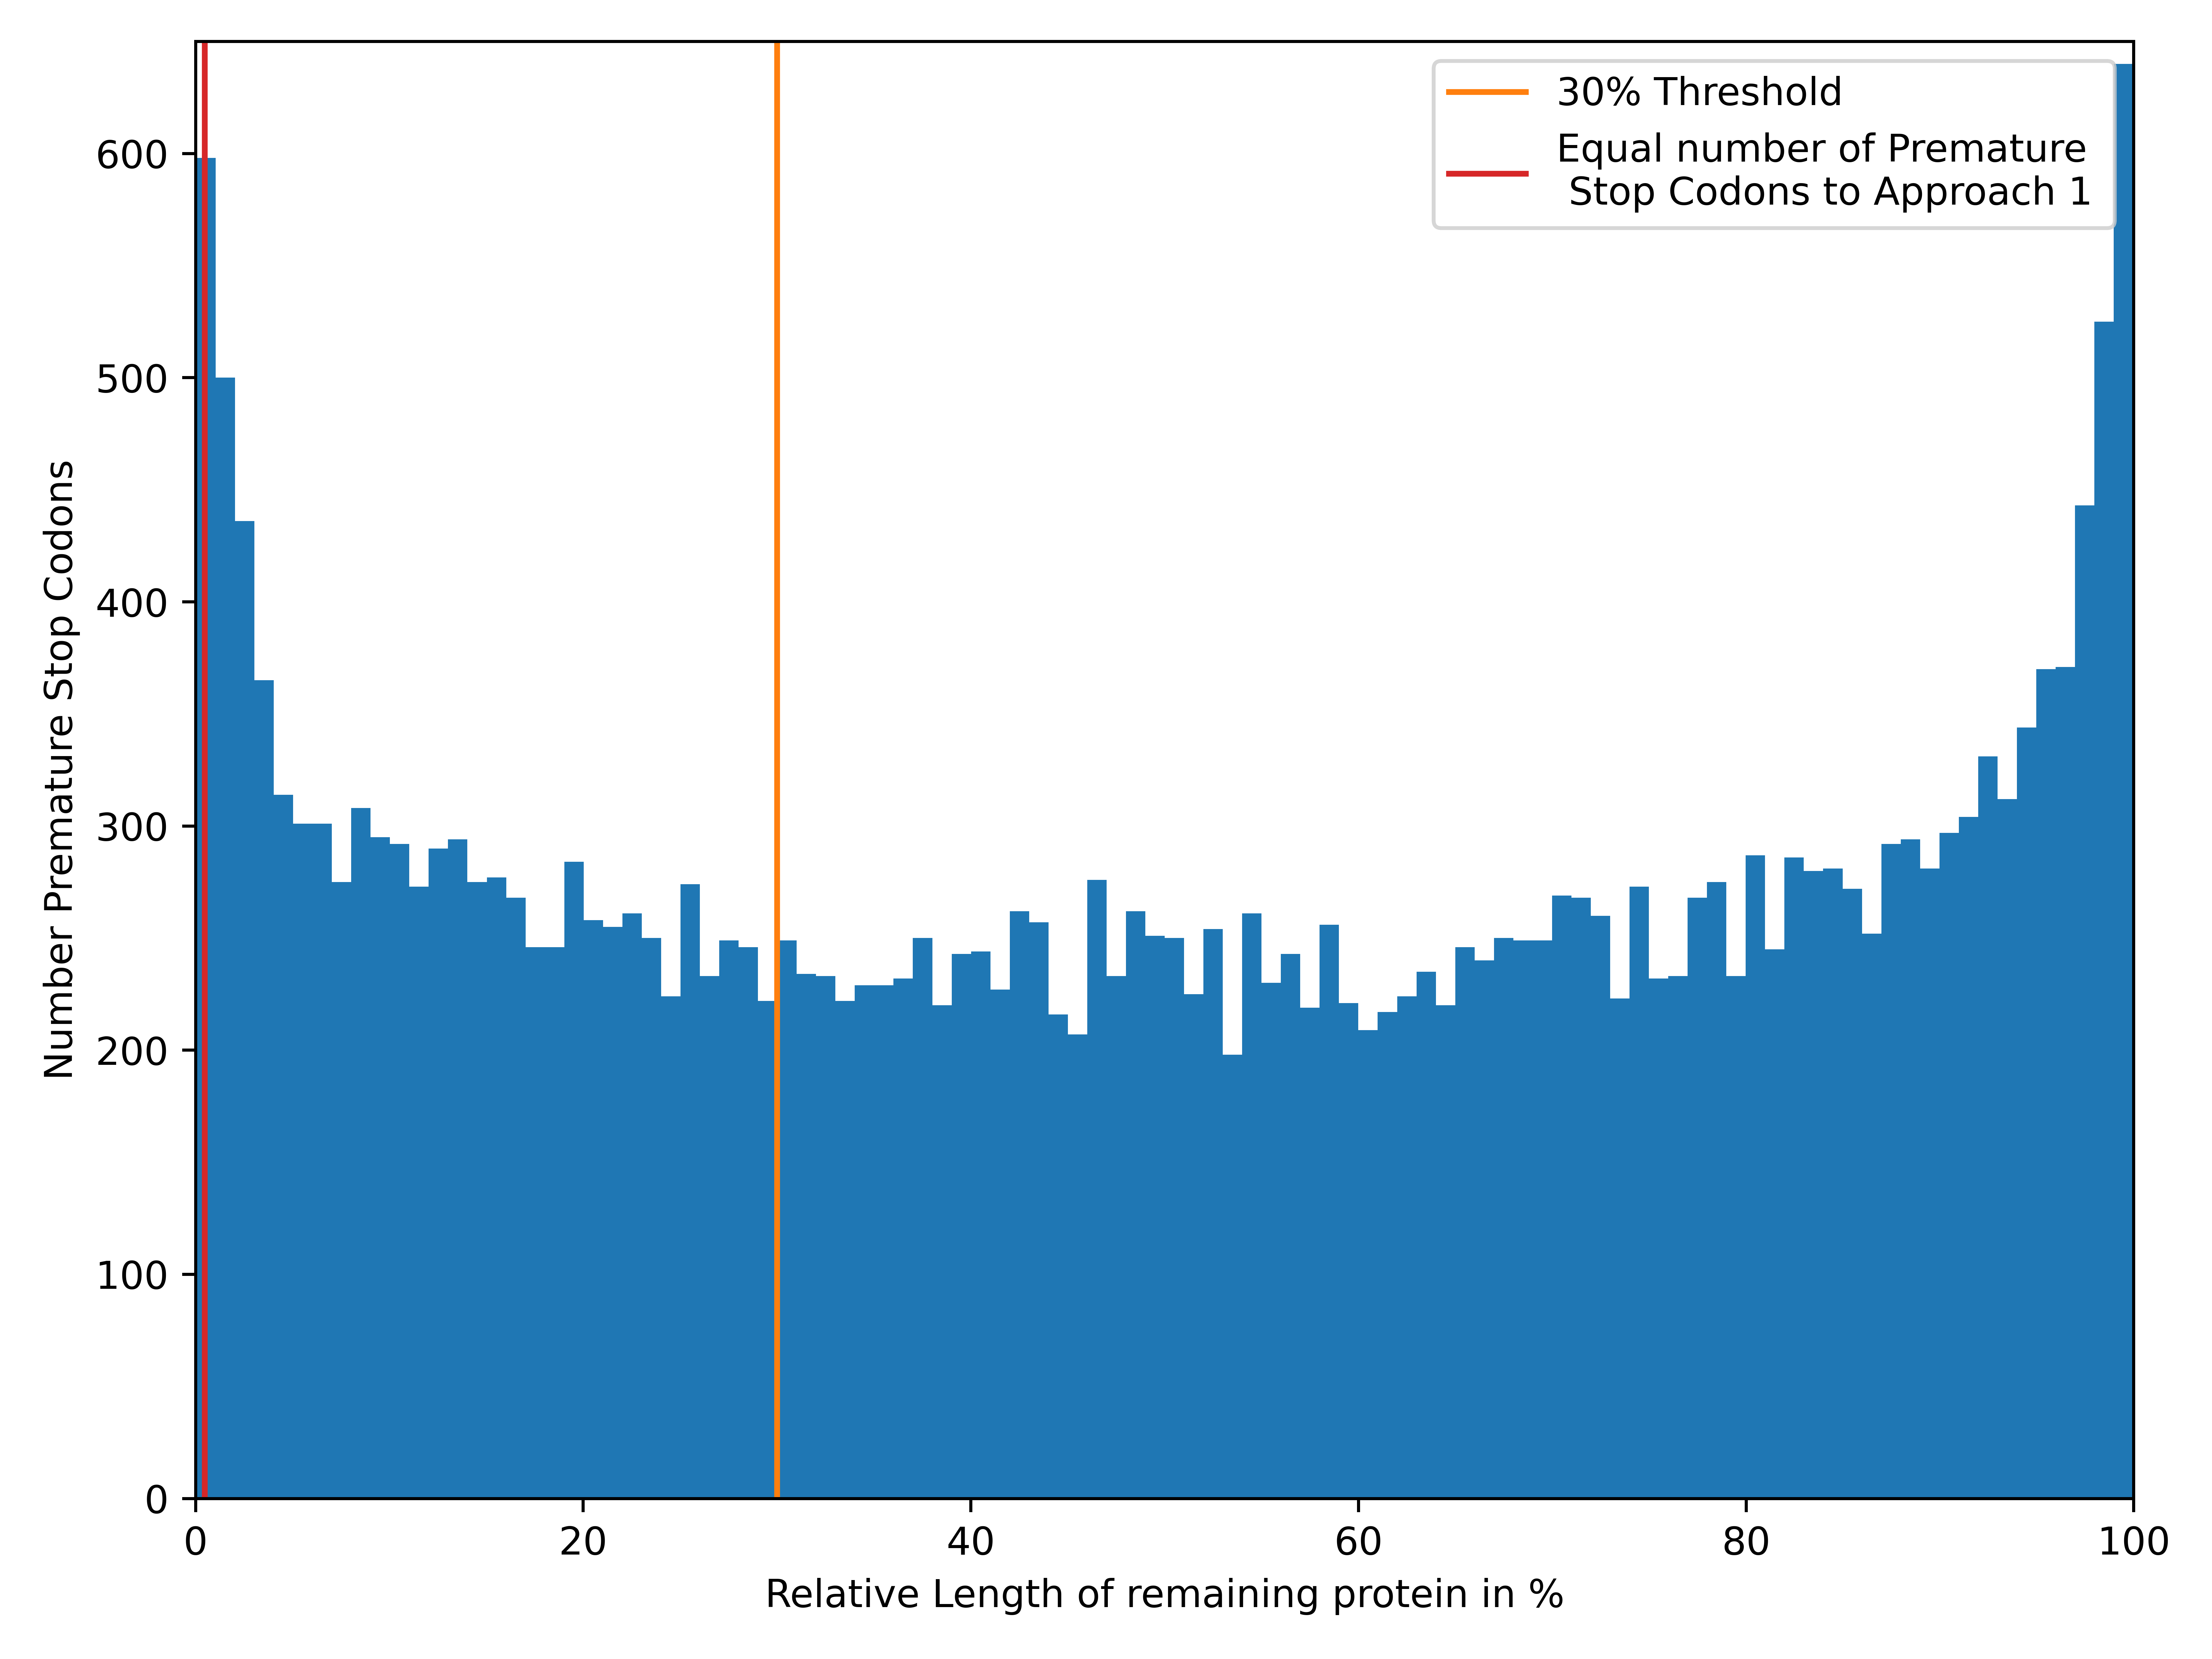
\includegraphics[width=0.8\textwidth]{images/Remaining_Length.png}
		\label{fig:Remaining_Length}
		\end{minipage}
	\end{figure}
\end{frame}
\begin{frame}{Comparison of both approaches}
	\textbf{Equal numbers of premature stop codons in high confidential dataset}
	
	\vspace{3mm}

	\begin{figure}[tb]
		\centering
		\begin{minipage}[h]{1\textwidth}
		\centering
		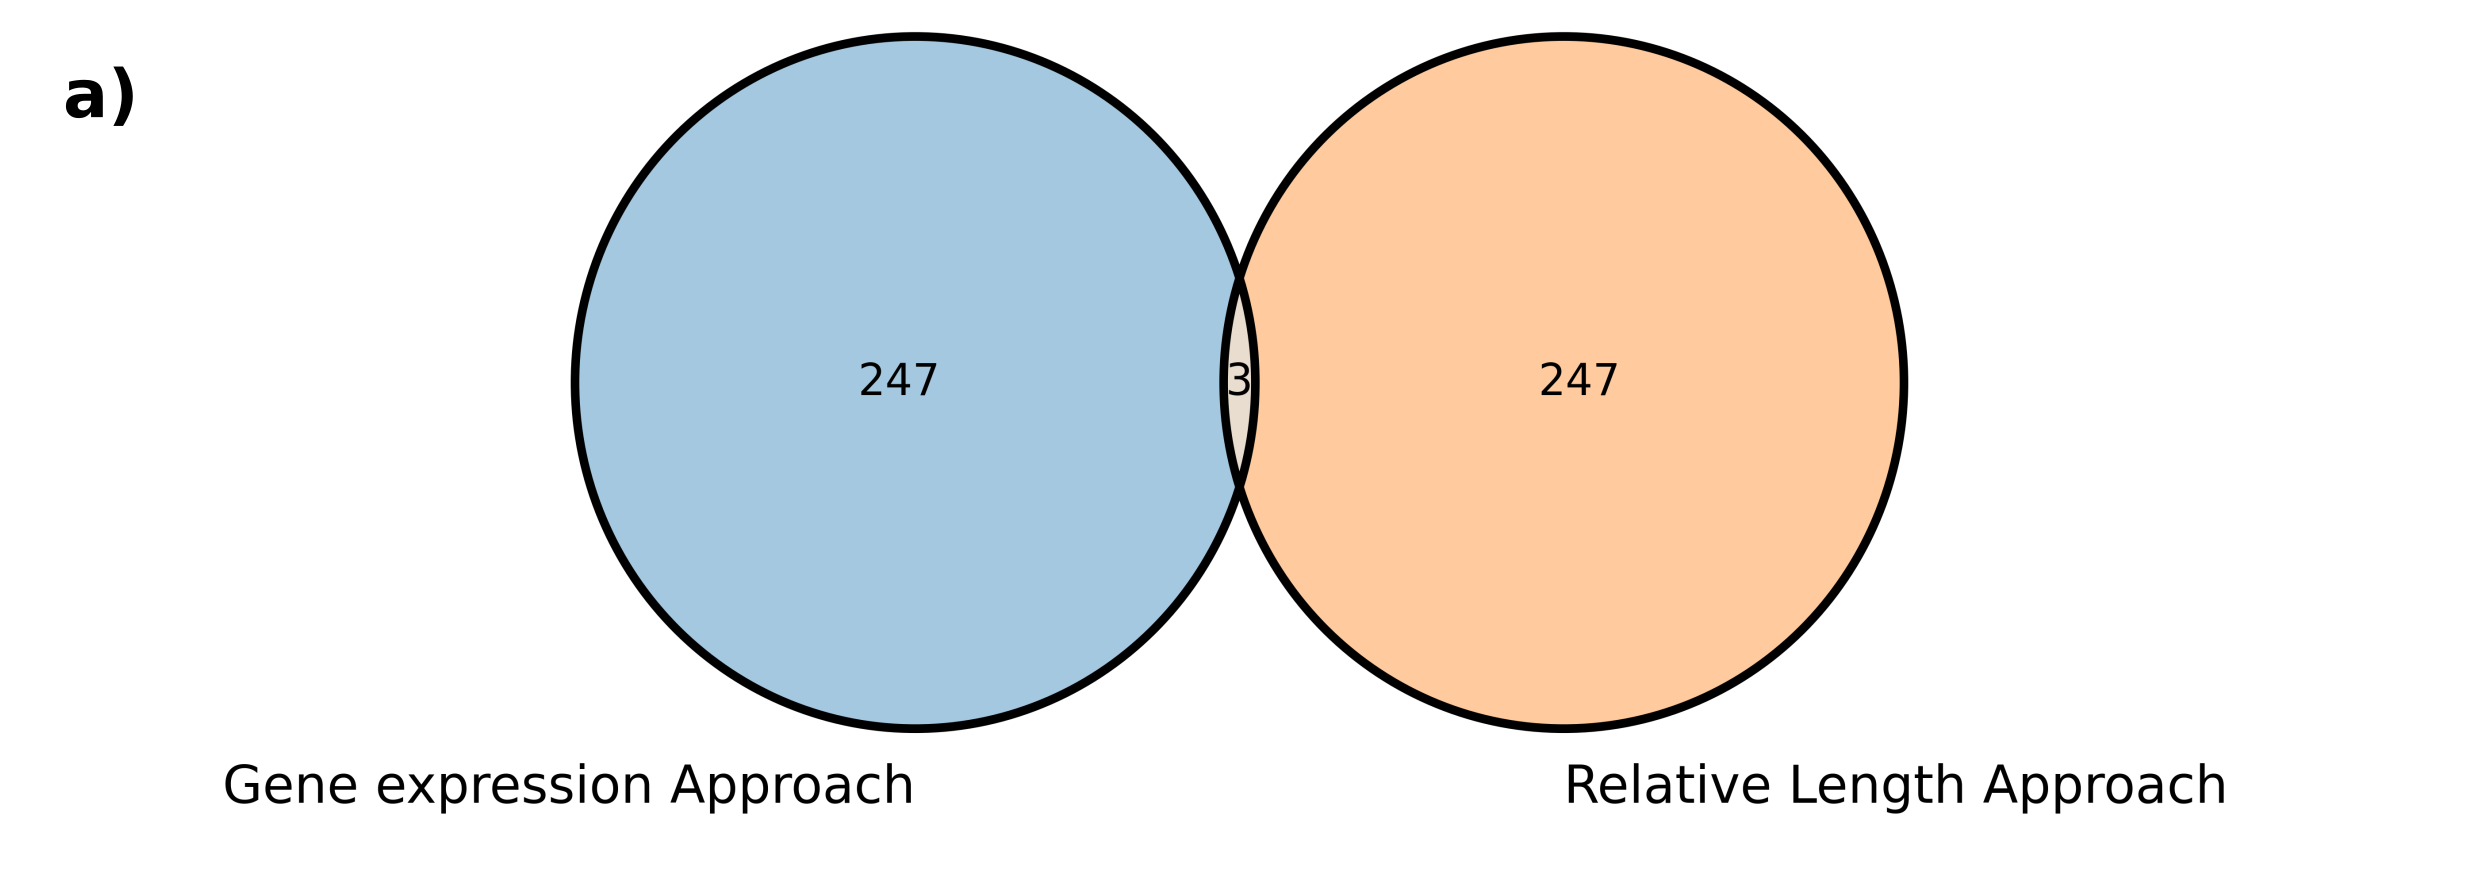
\includegraphics[width=0.8\textwidth]{images/Venn_Diagramm_small.png}
		\label{fig:Venn_Diagramm_small}
		\end{minipage}
	\end{figure}
\end{frame}
\begin{frame}{Comparison of both approaches}
	\textbf{30\% remaining length compared to bonferroni Significant decreased gene expression}
	
	\vspace{3mm}
	 
	\begin{figure}[tb]
		\centering
		\begin{minipage}[h]{1\textwidth}
		\centering
		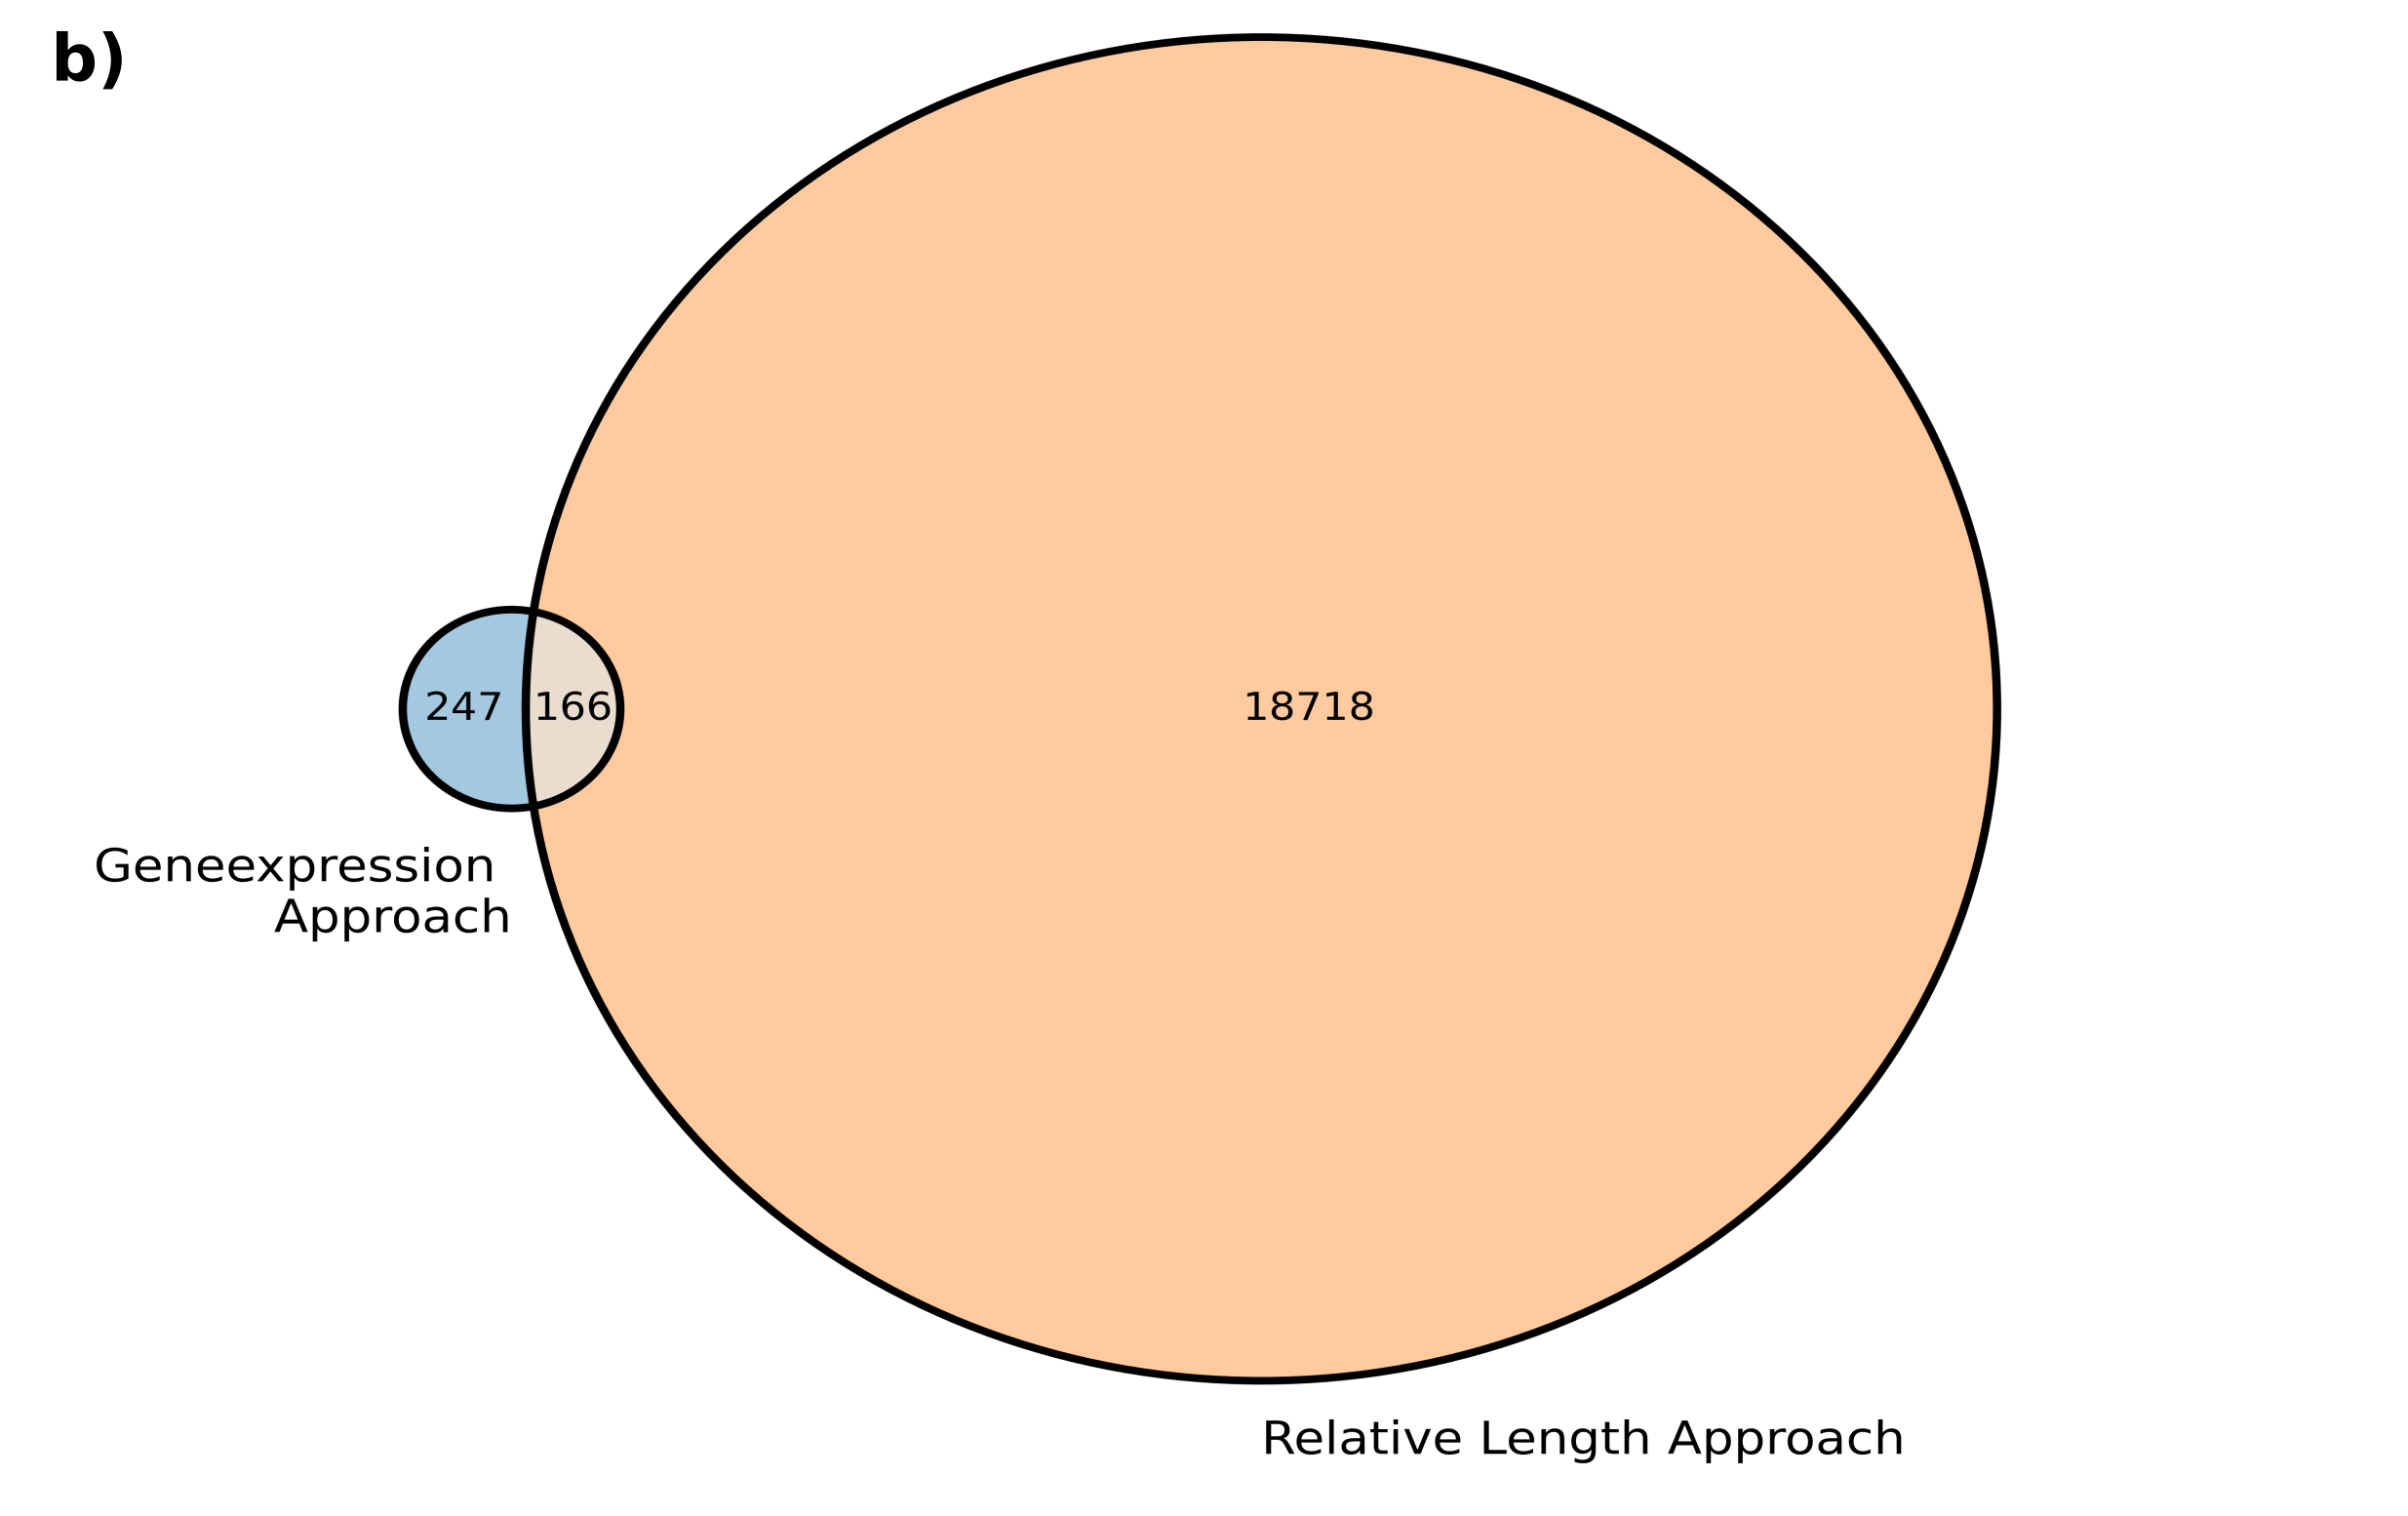
\includegraphics[width=0.8\textwidth]{images/Venn_Diagramm_big.png}
		\label{fig:Venn_Diagramm_big}
		\end{minipage}
	\end{figure}
\end{frame}
\section{Interactions between premature stop codons}
\begin{frame}[plain]
    \vfill
    \centering
    \begin{beamercolorbox}[sep=8pt,center,shadow=true,rounded=true]{title}
      \usebeamerfont{title}\insertsectionhead\par%
      \noindent\rule{10cm}{1pt} \\
    \end{beamercolorbox}
    \vfill
\end{frame}

\begin{frame}{Workflow to study interactions}
	\begin{enumerate}
		\item Compression of the list of single premature stop codons of the high confident dataset of gene expression approach to a gene based list of premature stop codons 
		\item Build interaction pairs of two between these gene based premature stop codons 
		\item Analyse the number of times, in which this pair is observed together in an accession 
		\item Calculate a hypergeometric test to statistically analyse if the number of cooccurrence we observe is significantly different from what we would expect as an expectation interval
	\end{enumerate}
\end{frame}
\begin{frame}{Coocurrence between premature stop codons}
	\begin{table}[tb]
		\label{tab:Coocurrence}
		\centering
		\begin{tabular}{|l|l|l|}
		\hline
		\textbf{p-value threshold} & \textbf{over-cooccurrence}  &  \textbf{under-cooccurrence}  \\ \hline
		0.05 & 19208 &  134 \\ \hline
		bonferroni-corrected & 1128 &  - \\ \hline
		\end{tabular}
		\end{table}
\end{frame}
\begin{frame}{Summary}
	\begin{itemize}
		\item Premature stop codons are distributed all over the 665 accessions of \textit{A. thaliana} and many hundreds of premature stop codon mutations occur for each accession
		\item By classifying premature stop codons based on their gene expression differences we find three categories 
		\item We use for further analysis as a high confidential dataset the premature stop codons which show bonferroni significant decreased gene expression 
		\item By studying pairs of interactions we found that specific premature stop codons are linked together 
	\end{itemize}
\end{frame}
\begin{frame}{Outlook}
	\begin{itemize}
	\item Control with synonymous and non-synonymous mutations
	\item Control of hypergeometric test by applying GWAS (Genome-wide association studies)
	\item Creating gene-regulatory networks based on our results to study the interaction between these linked pairs closer 
	\item Study the group of premature stop codons which result in a positive regulation, which means that they increase their gene expression more closely 
	\end{itemize}
\end{frame}
\end{document}